\documentclass{beamer}
\mode<presentation>
\usepackage{amsmath}
\usepackage{amssymb}
%\usepackage{advdate}
\usepackage{adjustbox}
\usepackage{subcaption}
\usepackage{enumitem}
\usepackage{multicol}
\usepackage{mathtools}
\usepackage{listings}
\usepackage{url}
\def\UrlBreaks{\do\/\do-}
\usetheme{Boadilla}
\usecolortheme{lily}
\setbeamertemplate{footline}{
  \leavevmode%
  \hbox{%
    \begin{beamercolorbox}[wd=.9\paperwidth,ht=2.25ex,dp=1ex,left]{author in head/foot}%
      \hspace{1em} Balaji B % Your name here
    \end{beamercolorbox}%
    \begin{beamercolorbox}[wd=.1\paperwidth,ht=2.25ex,dp=1ex,right]{author in head/foot}%
      \insertframenumber{} / \inserttotalframenumber\hspace*{2ex}
    \end{beamercolorbox}}%
}
\setbeamertemplate{navigation symbols}{}

\providecommand{\nCr}[2]{\,^{#1}C_{#2}} % nCr
\providecommand{\nPr}[2]{\,^{#1}P_{#2}} % nPr
\providecommand{\mbf}{\mathbf}
\providecommand{\pr}[1]{\ensuremath{\Pr\left(#1\right)}}
\providecommand{\qfunc}[1]{\ensuremath{Q\left(#1\right)}}
\providecommand{\sbrak}[1]{\ensuremath{{}\left[#1\right]}}
\providecommand{\lsbrak}[1]{\ensuremath{{}\left[#1\right.}}
\providecommand{\rsbrak}[1]{\ensuremath{{}\left.#1\right]}}
\providecommand{\brak}[1]{\ensuremath{\left(#1\right)}}
\providecommand{\lbrak}[1]{\ensuremath{\left(#1\right.}}
\providecommand{\rbrak}[1]{\ensuremath{\left.#1\right)}}
\providecommand{\cbrak}[1]{\ensuremath{\left\{#1\right\}}}
\providecommand{\lcbrak}[1]{\ensuremath{\left\{#1\right.}}
\providecommand{\rcbrak}[1]{\ensuremath{\left.#1\right\}}}
\theoremstyle{remark}
\newtheorem{rem}{Remark}
\newcommand{\sgn}{\mathop{\mathrm{sgn}}}
\providecommand{\abs}[1]{$\left \vert#1\right\vert$}
\providecommand{\res}[1]{\Res\displaylimits_{#1}} 
\providecommand{\norm}[1]{\lVert#1\rVert}
\providecommand{\mtx}[1]{\mathbf{#1}}
\providecommand{\mean}[1]{E$\left[ #1 \right ]$}
\providecommand{\fourier}{\overset{\mathcal{F}}{ \rightleftharpoons}}
%\providecommand{\hilbert}{\overset{\mathcal{H}}{ \rightleftharpoons}}
\providecommand{\system}{\overset{\mathcal{H}}{ \longleftrightarrow}}
	%\newcommand{\solution}[2]{\textbf{Solution:}{#1}}
%\newcommand{\solution}{\noindent \textbf{Solution: }}
\providecommand{\dec}[2]{\ensuremath{\overset{#1}{\underset{#2}{\gtrless}}}}
\newcommand{\myvec}[1]{\ensuremath{\begin{pmatrix}#1\end{pmatrix}}}
\let\vec\mathbf

\lstset{
%language=C,
frame=single, 
breaklines=true,
columns=fullflexible
}

\numberwithin{equation}{section}
\title{Matgeo 9-9.3-9}
\author{EE24BTECH11010-Balaji B}
\date{\today} 

\begin{document}

\begin{frame}
\titlepage
\end{frame}

\section*{Outline}
\begin{frame}
\tableofcontents
\end{frame}

\section{Question}
\begin{frame}
\frametitle{Question}
If the area of the region rounded by the curve $y^2 = 4ax$ and the line $x = 4a $ is $\frac{256}{3}$ sq.units then using integration, find the value of $a$ , where $a > 0$.
\end{frame}

\section{Solution}
\subsection{Parameters}
\begin{frame}
\frametitle{Parameters}
The parameters for the problem are given as follows:
\begin{table}[H]
    \centering
    \begin{tabular}[12pt]{ |c| c| c|c|c|c|}
    \hline
    $X$ & 1 & 2 & 3 & 4 & 5 \\
    \hline
    $P(X)$ & $K$ & 2$K$ & 2$K$ & 3$K$ & $K$ \\
    \hline 
    \end{tabular} 

    \caption{Parameter Used}
    \label{tab1-1.9-6}
\end{table}

\end{frame}
\subsection{Intersection Points}
\begin{frame}
\frametitle{Intersection Points}
The equation of a parabola in Matrix form is
\begin{align}
\vec{x}^\top\vec{V}\vec{x} + 2\vec{u}^\top\vec{x} + f = 0
\end{align}
The equation of a line in vector form is
\begin{align}
\vec{x}&=\vec{h}+\kappa\vec{m}
\end{align}
For the given parabola $y^2=4ax$, The values of $\vec{V}$,$\vec{u}$,$f$ are
\begin{align}
\vec{V}&=\myvec{0 & 0\\0 & 1}\\
\vec{u}&=\myvec{-2a\\0}\\
f&=0
\end{align}
\end{frame}
\begin{frame}
    For the given line $x=4a$, The values of $\vec{h}$, $\vec{m}$ are
\begin{align}
\vec{h}&=\myvec{4a\\0}\\
\vec{m}&=\myvec{0\\1} 
\end{align}
Substituting the line equation in parabola equation gives the values of $\kappa$
\begin{align}
    \brak{\vec{h}+\kappa\vec{m}}^\top\vec{V}\brak{\vec{h}+\kappa\vec{m}} + 2\vec{u}^\top\brak{\vec{h}+\kappa\vec{m}} + f = 0 
\end{align}
{\scriptsize
\begin{align}
\brak{\myvec{4a\\0}+\kappa\myvec{0\\1}}^\top\myvec{0 & 0\\0 & 1}\brak{\myvec{4a\\0}+\kappa\myvec{0\\1}} + 2\myvec{-2a\\0}^\top\brak{\myvec{4a\\0}+\kappa\myvec{0\\1}} + 0 &= 0 
\end{align}}
\begin{align}
    \myvec{4a&\kappa}\myvec{0&0\\0&1}\myvec{4a\\\kappa}+2\myvec{-2a&0}\myvec{4a\\\kappa} &= 0
\end{align}
\end{frame}
\begin{frame}
    \begin{align}
        \myvec{4a&\kappa}\myvec{0\\\kappa}+2\brak{-8a^2} &= 0\\
        \kappa^2-16a^2&= 0\\
        \kappa_1&=4a\\
        \kappa_2&=-4a
    \end{align}
    The intersection points are
    \begin{align}
        \vec{x_1} &= \vec{h}+\kappa_1\vec{m}\\
\vec{x_1} &= \myvec{4a\\4a}\\
\vec{x_2} &= \vec{h}+\kappa_2\vec{m}\\
\vec{x_2} &= \myvec{4a\\-4a}
    \end{align}

\end{frame}
\subsection{Area Calculation}
\begin{frame}
\frametitle{Area Calculation}
The Area under the curve is given by
\begin{align}
A &= \int_{-4a}^{4a}\brak{\frac{y^2}{4a}}dy\\
A &= \brak{\frac{1}{4a}}\brak{\frac{(4a)^3 - \brak{(-4a)^3}}{3}}\\
A &= \brak{\frac{1}{12a}}\brak{128a^3}\\
A &= \frac{32a^2}{3}
\end{align}
\end{frame}
\subsection{Finding $a$}
\begin{frame}
\frametitle{Finding $a$}
The area of region bounded by the line $x=4a$ and the parabola $y^2=4ax$ is given as $\frac{256}{3}$ \\ 
Comparing the above area with the given area we get, the value of $a$ as  
\begin{align}
    \frac{32a^2}{3} = \frac{256}{3} \\ 
    a = 2\sqrt{2}
    \end{align}

\end{frame}
\subsection{Graph}
\begin{frame}
\frametitle{Graph}
\begin{figure}[h]
    \centering
    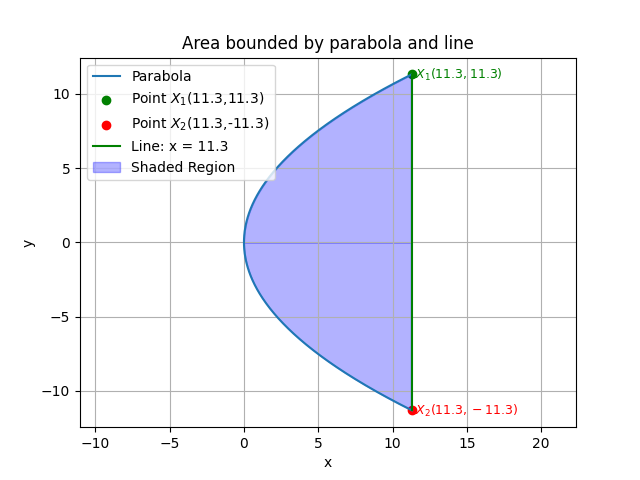
\includegraphics[width=\columnwidth]{figs/fig.png}
    \caption{Area bounded by  parabola and line}
\end{figure}
\end{frame}
\subsection{C Code}
\begin{frame}[fragile]
\frametitle{C Code}
\begin{lstlisting}[language=C]
#include <math.h>
#include <stdio.h>
#include <stdlib.h>
#include <string.h>
#include <sys/socket.h>
#include <netinet/in.h>
#include <unistd.h>

#include "libs/matfun.h"
#include "libs/geofun.h"

typedef struct 
{
    double **p;
}Point;

\end{lstlisting}
 \end{frame}
 \begin{frame}[fragile]
 \begin{lstlisting}[language = C]
 typedef struct 
{
    double **V;
    double **u;
    double f;
}Parabola;

void InitializePoint(Point *point)
{
    point->p = createMat(2,1);
}

void InitializeParabola(Parabola *parabola)
{
    parabola->V = createMat(2,2);
    parabola->u = createMat(2,1);
    parabola->f = 0;
}
 \end{lstlisting}
 \end{frame}
  \begin{frame}[fragile]
 \begin{lstlisting}[language = C]
void parab_y2_4ax_gen(FILE *fptr, Point *x1, Point *x2, double a, int num_points) 
{
    double tinit = (x1->p[0][0] / (2 * a));
    double tfinal = (x2->p[1][0] / (2 * a));

    Point coord;
    InitializePoint(&coord);
    if (tfinal > tinit)
    {
        for (double i = tinit; i <= tfinal; i += 1.0 / num_points) 
        {
            coord.p[0][0] = a*i*i;
            coord.p[1][0] = 2*a*i;
            fprintf(fptr,"%lf,%lf\n", coord.p[0][0], coord.p[1][0] );
        }
    }
    else
\end{lstlisting}
\end{frame}
\begin{frame}[fragile]
 \begin{lstlisting}[language = C]
 {
        for (double i = tfinal; i <= tinit; i += 1.0 / num_points)
        {
            coord.p[0][0] = a*i*i;
            coord.p[1][0] = 2*a*i;
            fprintf(fptr,"%lf,%lf\n", coord.p[0][0], coord.p[1][0] );
        }
    }
}

Point* intersect_of_parab_line(Parabola *parabola, Point *point_line, Point *slope)
{
    double m1 = slope->p[0][0];
    double m2 = slope->p[1][0];

    double h1 = point_line->p[0][0];
    double h2 = point_line->p[1][0];
\end{lstlisting}
\end{frame}

\begin{frame}[fragile]
\begin{lstlisting}[language = C]
double V1 = parabola->V[0][0];
    double V2 = parabola->V[1][0];
    double V3 = parabola->V[0][1];
    double V4 = parabola->V[1][1];

    double u1 = parabola->u[0][0];
    double u2 = parabola->u[1][0];

    double A = V1 * m1 * m1 + (V2 + V3) * m1 * m2 + V4 * m2 * m2;
    double B = 2 * (m1 * (V1 * h1 + V2 * h2 + u1) + m2 * (V3 * h1 + V4 * h2 + u2));
    double C = h1 * (V1 * h1 + V2 * h2) + h2 * (V3 * h1 + V4 * h2) + 2 * (u1 * h1 + u2 * h2) + parabola->f;

    if (B * B - 4 * A * C < 0) 
    {
        return NULL;
    }
    \end{lstlisting}
    \end{frame}
    
    \begin{frame}[fragile]
\begin{lstlisting}[language = C]
else
    {
        Point *intersection = malloc(2*sizeof(Point));
        InitializePoint(&intersection[0]);
        InitializePoint(&intersection[1]);

        if (B * B - 4 * A * C == 0) {
            double k = -B / (2 * A);
            intersection[0].p[0][0] = point_line->p[0][0] + k * slope->p[0][0];
            intersection[0].p[1][0] = point_line->p[1][0] + k * slope->p[1][0];
            return intersection;
        }
         else
        {
            double k1 = (-B + sqrt(B * B - 4 * A * C)) / (2 * A);
            double k2 = (-B - sqrt(B * B - 4 * A * C)) / (2 * A);

\end{lstlisting}
\end{frame}

  \begin{frame}[fragile]
\begin{lstlisting}[language = C]

intersection[0].p[0][0] = point_line->p[0][0] + k1 * slope->p[0][0];
            intersection[0].p[1][0] = point_line->p[1][0] + k1 * slope->p[1][0];
            intersection[1].p[0][0] = point_line->p[0][0] + k2 * slope->p[0][0];
            intersection[1].p[1][0] = point_line->p[1][0] + k2 * slope->p[1][0];
            return intersection;
            }
      }
}

int main()
{
    Parabola parabola;
    Point p1;
    Point p2;
 \end{lstlisting}
    \end{frame}
    
     \begin{frame}[fragile]
\begin{lstlisting}[language = C]
    Point slope;
    Point point_line;

    InitializeParabola(&parabola);
    InitializePoint(&p1);
    InitializePoint(&p2);
    InitializePoint(&slope);
    
    parabola.V[0][0] = 0;
    parabola.V[0][1] = 0;
    parabola.V[1][0] = 0;
    parabola.V[1][1] = 1;
    parabola.u[0][0] = 0;
    parabola.u[1][0] = -4*sqrt(2);
    parabola.f = 0;
    
    point_line.p[0][0] = 8*sqrt(2);
    point_line.p[1][0] = 0;
\end{lstlisting}
\end{frame}

 \begin{frame}[fragile]
\begin{lstlisting}[language = C]
    slope.p[0][0] = 0;
    slope.p[1][0] = 1;

    Point *intersection = intersect_of_parab_line(&parabola, &point_line, &slope);

    p1.p[0][0] = intersection[0].p[0][0];
    p1.p[1][0] = intersection[0].p[1][0];

    p2.p[0][0] = intersection[1].p[0][0];
    p2.p[1][0] = intersection[1].p[1][0];
    
    FILE *fptr = fopen("parab.txt", "w");
    if (fptr == NULL) 
    {
        printf("Error opening file!\n");
        return 1;
 \end{lstlisting}
    \end{frame}

 \begin{frame}[fragile]
\begin{lstlisting}[language = C]
}

    parab_y2_4ax_gen(fptr, &p1, &p2, -parabola.u[1][0] / 2, 150);
    fclose(fptr);
    return 0;

}

\end{lstlisting}
\end{frame}

\subsection{Python Code}
\begin{frame}[fragile]
\frametitle{Python Code}
\begin{lstlisting}[language = Python]

import numpy as np
import matplotlib.pyplot as plt
import math

# Load points from the file
points = np.loadtxt('parab.dat', delimiter=',', max_rows=len(list(open("./parab.dat")))-1)

# Extract x and y values
x = points[:, 0]
y = points[:, 1]

# Define points A, B, C, D
x1 = np.array([11.3, 11.3])
x2 = np.array([11.3, -11.3])

\end{lstlisting}
\end{frame}

\begin{frame}[fragile]
\begin{lstlisting}[language = Python]
# Plot the parabola
plt.plot(x, y, label='Parabola')

# Plot the specific points
plt.scatter(x1[0], x1[1], color='green', marker='o', label='Point $X_1$(11.3,11.3)')
plt.scatter(x2[0], x2[1], color='red', marker='o', label='Point $X_2$(11.3,-11.3)')

# Define the line equation x = 8*\sqrt2
line_y = np.linspace(min(y), max(y), 400)
line_x = line_y * 0 + 11.3

# Plot the line x=11.3
plt.plot(line_x, line_y, color='green', label='Line: x = 11.3')

plt.text(x1[0] + 0.2, x1[1] - 0.3, '$X_1(11.3,11.3)$', color='green', fontsize=9)
\end{lstlisting}
\end{frame}

\begin{frame}[fragile]
\begin{lstlisting}[language = Python]
# Fill the closed region between the parabola and the line x=11.3
plt.fill_between(x, y, where=(x <= 11.3), color='blue', alpha=0.3, label='Shaded Region')

# Label the axes and add a title
plt.xlabel("x")
plt.ylabel("y")
plt.title("Parabola, Line, and Points $X_1$ & $X_2$")
plt.grid(True)
plt.legend(loc='upper left')
plt.axis('equal')

# Save the plot to a file
plt.savefig('../figs/fig.png')
plt.show()\end{lstlisting}
\end{frame}

\end{document}